\section{Numerical Experiments}
%We provide numerical evidence supporting our conclusions.


\subsection{Simulating Theorem \ref{thm:char}}\label{subsec:lemma_sims}
In the proof of Theorem \ref{thm:char} we utilize Lemma
\ref{lemma:free} to construct D-optimal designs. We implement this
construction with the goal of testing numerically how prevalent are
clustered designs. To this end, we would like to generate random prior
eigenvalues $\lambda_j$, fix $m$ and $k$, find what a D-optimal
$\opt^*\opt$ should be, and then utilize the construction of
Theorem~\ref{thm:char} and Lemma~\ref{lemma:free} to find $\opt$.


To simplify things, we directly generate $\opt^*\opt$. We iterate over
the number of measurements $m \in \{4,\dots, 24\}$, and for every $m$
we then iterate over $k:=\rank \opt^*\opt \in \{2,\dots, m-1\}$. For
each pair $m,k$ we repeat the following steps $N=5000$ times:
\begin{enumerate}
\item Generate random diagonal $D\in \mathbb{R}^{k\times k}$ with
  entries $\log (d_i) \sim \mathcal{N}(50,15)$.
\item Normalize $D$ that $\ttr D = m$.
\item Conjugate $D$ by a random orthogonal matrix to form a positive
  semi-definite $M := UDU^t \in \mathbb{R}^{k\times k}$. This $M$
  represents $\opt^*\opt$.
\item Apply the construction of Lemma \ref{lemma:free} to calculate
  $A$ such that $AA^t = M$, where $A$ has unit norm columns. $A^t$ is
  our optimal design $\opt$.
\item Since $A^t$ corresponds to $\opt$, its columns correspond to
  measurement vectors. We call $A$ "clustered" if $A$ has two or more
  identical columns (up to some numerical precision threshold,
  i.e.~$10^{-5}$).
\end{enumerate}
We then calculate the fraction of clustered designs of the simulations
we ran, for each pair $m,k$. Clusterization occurred at high rates
($>99.9\%$) whenever $m-k > 1$; see Fig.~\ref{fig:sim_AAt}. Hence, in
these simulations, clusterization is a generic property. However, when
$m-k = 1$, clusterization does not occur. We do not why this is so.

\begin{figure}
    \centering
    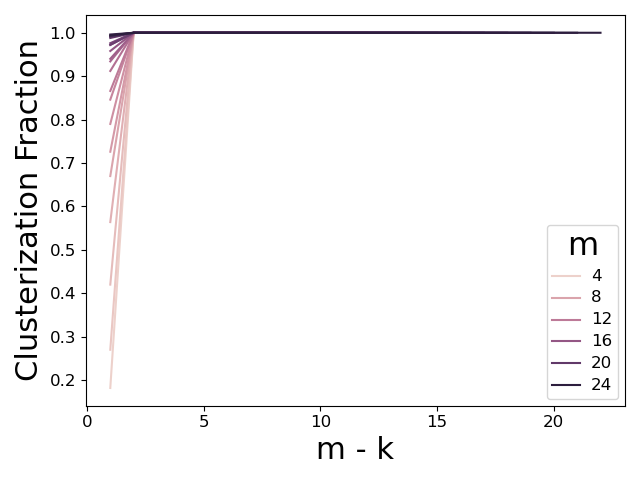
\includegraphics[height=0.5\textwidth]{figs/simulations.png}
    \caption{Fraction of clustered $A$ for $AA^t = M$ and $M$
      generated randomly (see text and repository for details on
      generating $M$). It is evident that when $m-k > 1$ clusterization
      is prevalent, whereas for lower $m-k$ clusterization is not.}
  \label{fig:sim_AAt}
\end{figure}

Full results are located in the \texttt{simulations.csv} file within
the accompanying \href{https://github.com/yairdaon/OED}{repository}.
Code implementing the experiments described above is located in module
\texttt{zeros.py} of said repository. Runtime should be less than 30
minutes on any reasonably modern laptop (it took 12 minutes on the
author's laptop).





\subsection{Correlated errors}\label{subsec:corr_errors_sims}
In order to verify the results of Section \ref{section:non_vanishing},
we run simulations of the inverse problem of the 1D heat equation with
nonvanishing model error \(\modcov = \prcov^2 \). Indeed, including
model correlation pushes measurements apart, see
Fig.~\ref{fig:corr_errors}. Code generating Fig.~\ref{fig:corr_errors}
is located in module \texttt{clusterization.py} in the accompanying
\href{https://github.com/yairdaon/OED}{repository}.

\begin{figure}
    \centering
    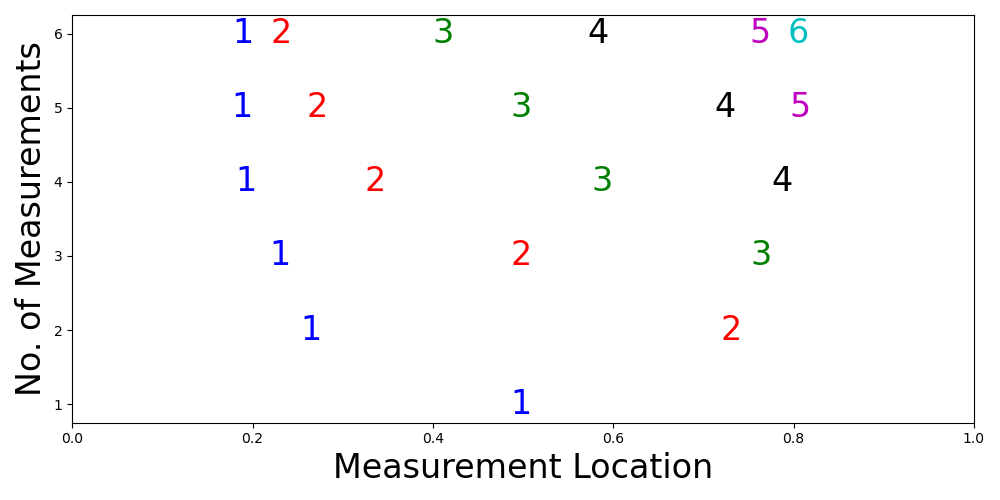
\includegraphics[height=0.5\textwidth]{figs/dst_modelError4.png}
    \caption{Model correlation mitigates clusterization. We add a
      model correlation term to the error terms in the 1D heat
      equation inverse problem. As expected, measurements are pushed
      away owing to the model error term.}
  \label{fig:corr_errors}
\end{figure}


%% \subsection{Implementing the 1D heat equation}
%% The Laplacian $\Delta$ is a Fourier multiplier \cite{stein2009}, so
%% our implementation proceeds in frequency space. When we utilize the
%% homogeneuous Dirichlet boundary condition, the eigenvectors of
%% $\Delta$ are sines $\ev_n(x) = \sin(\pi n x), n=1,2,3,\dots$, whereas
%% for the homogenoeous Neumann boundary condition the eigenvectors are
%% cosines $\cos(\pi n x)$. Implementing point evaluations in Fourier
%% space

